%PIP-412035RC020
\documentclass[reprint,amsmath,amssymb,aps,prb,footinbib,floatfix]{revtex4-2}
\bibliographystyle{apsrev4-2}
%\usepackage{afterpage}
\usepackage{blindtext}
\usepackage[rgb]{xcolor}
%\usepackage[twocolumn=true,includehead=false,left=.75in,right=.75in,top=.75in,bottom=.75in]{geometry}
%\usepackage[letterpaper, portrait, twocolumn, twoside, left=2cm, hmarginratio=2:1, includemp, marginparwidth=43pt, bottom=1cm, foot=.7cm, includefoot, textheight=11cm, heightrounded, columnsep=1cm, dvips, verbose]{geometry}
\definecolor{Cred}{RGB}{208, 32, 46}
\usepackage[firstpage=true]{background}
\usetikzlibrary{calc}
%\usepackage{tikz}
\backgroundsetup{angle = 0, scale = 1, vshift = 0pt, opacity=1,
  contents = {\begin{tikzpicture}[overlay,remember picture]
    \node at (0,0) {\includegraphics[scale=1]{RC_def.pdf}};
\end{tikzpicture}
}
}
%    \draw (3.4in,3.75in) node[inner sep=0] {\includegraphics[width=1in]{arrow.pdf}};
%    \draw (3.5in,3.85in) node[rotate=-90] {\scshape{Editor's}};
%    \draw (3.5in-\baselineskip,3.85in) node[rotate=-90] {\scshape{Suggestion}};
%\end{tikzpicture}

\usepackage{graphicx} % Required for inserting images
\usepackage{mathtools} % Useful for a bunch of math stuff
\usepackage{cleveref} % Use for better cross-references
\usepackage[caption=false]{subfig} % For sub-figures
\usepackage{booktabs} % For nicer looking tables
\usepackage[twoside]{fancyhdr}
\usepackage{appendix}

\usepackage{placeins}




\fancypagestyle{plain}{%
%\setlength{\headheight}{60pt}
\fancyhead[L,C]{}
\fancyhf{}
\fancyhead[R]{\raisebox{.6cm+1pt}{\textbf{Rapid Communication}}}
\fancyhead[L]{ \raisebox{.6cm+1pt}{\scshape{Editor's Suggestion}\vspace{12pt}}}
\fancyhead[C]{\raisebox{.6cm}{\large\scshape{CARTHAGE}}\hspace{0.2cm}\includegraphics[height=1.5cm]{Logo.pdf}\hspace{0.1cm}\raisebox{.6cm}{\large\scshape{COLLEGE 
 }}}
\fancyfoot[C]{\thepage}
\renewcommand{\headrulewidth}{0pt}
\renewcommand{\footrulewidth}{0pt}
}
\usepackage{printlen}


\pagestyle{fancy}
\fancyhf{}
\fancyheadinit{\setlength{\headheight}{20pt}}
\fancyhead[RO,LE]{\textbf{Rapid Communication}}
\fancyhead[LO,RE]{\textit{Phys. in Prog.} \textbf{2} (Feb. 2026)}
\fancyhead[C]{ \large \scshape{PHYSICS IN PROGRESS}}
\fancyfoot[C]{\thepage}
\renewcommand{\headrulewidth}{0.4pt}
\renewcommand{\footrulewidth}{0pt}

% These are packages I am using in this document
\usepackage{siunitx}

% Everything up to here is the 'document preamble'

\begin{document} 

\vspace*{25pt}

\title{Reflecting on microwaves with Lloyd's mirror}
\author{Skylar Farr}
\affiliation{%
Department of Physics and Astronomy,  Carthage College, 2001 Alford Park Drive, Kenosha, WI 53140, USA
}%
\collaboration{Received January 29, 2026, Published online February 5, 2026}
\begin{abstract}
    The wavelength of a microwave transmitter was determined by using a method of interferometry called Lloyd's Mirror. This method consists of a transmitter, reflector, and a receiver. By relating the total path a wave travels, to the distance of a reflector away from the wave, the wavelength of said microwave can be calculated using a linear regression. Two sets of data taken are consistent in showing distance does not change wavelength despite the imprecision of the results when compared to the recorded wavelength of the microwave transmitter. Outside influences creating additional reflection are likely the cause of this imprecision.
\end{abstract}


\maketitle
%\thispagestyle{plain}
\section{Introduction}
    Interferometry is a term used to describe the process in which the interference of waves are measured in order to determine various forms of data. This process has been used for many years to detect different variables and physical interactions. A popular example is from American Physicist Albert A. Michelson who created the Michelson Interferometer to measure the effects of Earth's movement on the speed of light. This experiment, fueled by curiosity, ended up showing the lack of existence of what Michelson thought was a medium surrounding the Earth, known as the aether \cite{ranzan2018history}. The Michelson interferometer is not the only use of this technology; it is also used in something called Lloyd's Mirror. This technique was made by Irish physicist Humphery Lloyd to learn more about the wave nature of light. However, unlike the original experiment, the specific set up for this experiment uses electromagnetic waves, EM waves, rather than light \cite{bromwich1919x}. Despite the difference in the type of waves, this method works by measuring the interference of waves in order to determine constants, such as the wavelength of the wave being used.

    Today, some other more common uses of interferometry and, more specifically, Lloyd's mirror are optical measurement, radio astronomy, and underwater acoustics. All of these applications put into use the different aspects of Lloyd's mirror, like understanding reflection and refraction of waves, being able to apply transformations to waves, and understanding constructive and destructive interference.


\section{The Experiment}
     Now that the some general information on interferometry has been laid out, it's time to understand Lloyd's Mirror more in depth. As stated above, it works by measuring the interference of waves. There are different interactions that happen between the waves to create interference. The first kind being constructive interference. This is when two waves align in the same phase to combine and become amplified. The second type is destructive interference where the two waves become out of phase and begin to cancel each other out. If two waves are $180^\circ$ out of phase, it is possible for them to completely cancel each other out. For the purposes of this lab, the waves were measured when they were in a state of constructive interference, or at the peak of their wavelength. The purpose for measuring these waves is to determine the wavelength based on the intensity of said waves which is determined by how their constructive and destructive interference changes.
     
     The set up of this experiment consists of the PASCO Microwave Transmitter WA-9801 and Microwave Receiver WA-9800, and other elements of the PASCO Microwave Optics System (WA-9314C) including component holders, metal reflectors, the fixed arm assembly, and the goiniometer. The receiver is equipped with a current sensor with a multiplier and sensitivity dial to be able to read the intensity of the waves it receives. For this experiment this display was simply used as a reference to be able to note the constructive and destructive interference of the waves. Both the transmitter and receiver are positioned along a meter stick with the goniometer in the center to allow for ease in adjustment of the angles of the transmitter and receiver. Additionally, the fixed arm assembly is placed onto the degree plate to be able to position the metal reflector plate. When all the equipment is set up, the transmitter and receiver should be directly across from each other with the openings facing each other and the reflector plate should be slightly offset, facing inward, while positioned at an equidistant point between the two, as seen in Figure \ref{schematic}.

     \begin{figure}
         \centering
         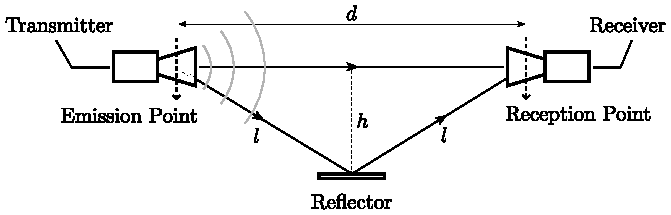
\includegraphics[width=1\linewidth]{Lab 4 Schematic.pdf}
         \caption{A schematic of the experimental setup containing an EM wave transmitter and receiver set up at distance $d$ apart, and a reflector plate at distance $h$ from the equidistant point between the two devices. The total path traveled by the wave is noted by $l$.}
         \label{schematic}
     \end{figure}

    The values being measured are the distance from the transmitter to the center of the goniometer $d$, and the distance of the reflector from the center point of the goniometer to the metal reflector $h$ as its distance changes with respect to the changing intensity of the waves. The values of eight different maxima of the wave intensity was measured at two different distances $d$. The equation to determine the wavelength from these values is
    \begin{equation}
        2l-d=n\lambda,
    \end{equation}
    where $2l$ is the total path traveled by the wave, $n$ is the number of waves or "fringes" that have been measured out from the first maximum point, and $\lambda$ is the wavelength. To be able to solve the equation, the value $2l$ must be found first. This can be done by using the Pythagorean theorem,
    \begin{align}
        a^2+b^2&=c^2, &  c&=\sqrt{a^2+b^2}.
    \end{align}
    After obtaining the value of $2l$ a linear regression can be performed on the data to plot the number of fringes vs. the total length traveled where the slope is the wavelength. This fit along with error bars is seen in figure \ref{fig:graph}. The estimated uncertainty of the distance of the reflector from the goniometer $h$ is $\pm0.5$ cm. When adjusting that distance, the dial displaying the current was not incredibly sensitive, so slight adjustments of the reflector often made little to no difference in the maximum intensity being displayed. This caused a lot of back and forth movement of the reflector to get a best estimate for the peak of the intensity and that back and forth movement often varied by about 0.5 cm.
    
    \begin{figure}
        \centering
        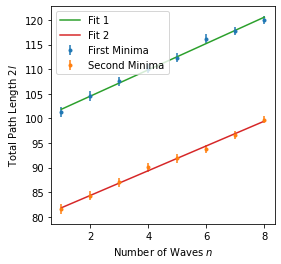
\includegraphics[width=0.8\linewidth]{Lloyd's Mirror Graph.png}
        \caption{Number of fringes vs. total path length the wave traveled. The slope of the fit line represents the wavelength of the microwaves emmited by the transmitter.}
        \label{fig:graph}
    \end{figure}

    As mentioned above, there were two sets of data taken, one where the distance between the transmitter and receiver was $d_1=100$ cm, and the other where $d_2=80$ cm. The goal with taking two sets of data was to see how distance affects the wavelength, while knowing that it should not. After plotting both data sets, the measured wavelengths for $d_1$ and $d_2$ are $\lambda_1=2.68$ cm and $\lambda_2=2.52$ cm. Taking into account the estimated uncertainty $\pm0.5$ cm, which is the same for both data sets, and performing an error analysis, the final uncertainty of the wavelengths is, $\delta=\pm0.08$ cm, making the final values $\lambda_1=2.68\pm0.08$ cm and $\lambda_2=2.52\pm0.08$ cm. The recorded wavelength of the microwaves emitted from the PASCO transmitter is $\lambda=2.85$ cm \cite{griffith}.
    
    Although these data are consistent within the data sets and despite the difference in distances between the transmitter and the receiver, figure \ref{fig:graph} still shows a linear relationship between the two data sets, the precision of the data compared to the recorded value of PASCO is significantly different. This is likely due to external interference and reflection from objects other than the receiver. If the person recording the data and moving the reflector recorded the maxima while positioned near or behind the reflector, that person would also act as a reflector. If the experiment was set up on an inconsistent surface, the adjustment of the reflector could have been inaccurate. This leads to the belief that the significant difference in the recorded vs. measured values has to do with some external factor since the results are consistent.


\section{Conclusion}
    This experiment was both successful and unsuccessful. The data gathered was consistent in displaying the linear relationship between distance the wave traveled and the number of fringes passed, and the results of the slope for both data sets accurately displayed the data, but the data was still imprecise to the recorded values of the transmitter. As mentioned above, this was likely caused by the person recording the data creating additional reflections or the condition of whatever surface the experiment was performed on. When performing data analysis, this potential error was not taken into consideration as the conditions in which all of the data was taken was consistent, meaning the data would be accurate within the sets taken and the amount of additional reflection would be the same for both data sets.

    In the future if this experiment were to be replicated, an important recommendation would be to find a smooth surface, along with finding a way to reduce any additional reflection. This could mean moving the reflector very slightly and backing away from the experimental set up to observe and record the status of the intensity, rather than remaining directly next to the equipment. This process may be more tedious as it will take many more iterations of adjustment, but the results would be more precise. Again, despite being imprecise, the data is still accurate and it correctly displays the relationship between distance and wavelength.


\section{Acknowledgments}
     This lab was completed with the collaboration from lab partner Brookelyn Velmont. Additionally, this research would not have been made possible without funding from the Carthage College Physics and Astronomy Department along with assistance from Dr. Joseph Anderson.

\section*{Data Availability Statement}
A Jupyter notebook containing all the experimental data, data analysis, figure generation, and additional information on uncertainty analysis can be found in the supplemental materials. \footnote{See online article posting for access to supplemental material.}


%\bibliographystyle{unsrt}
\bibliography{bib}

\end{document}